\documentclass[11pt,a4paper]{article}

\usepackage[T1]{fontenc}
\usepackage[utf8]{inputenc}
\usepackage{lmodern}
\usepackage{geometry}
\geometry{margin=2.5cm}

\usepackage{graphicx}
\usepackage{hyperref}
\usepackage{amsmath}
\usepackage{enumitem}
\usepackage{caption}
\usepackage{float} % Required for the [H] 'Force Here' placement

\usepackage{listings}
\usepackage{xcolor}

\definecolor{steelBlue}{rgb}{0.10, 0.25, 0.60}
\definecolor{slateGreen}{rgb}{0.20, 0.45, 0.30}
\definecolor{brickRed}{rgb}{0.70, 0.20, 0.20}
\definecolor{charcoal}{rgb}{0.15, 0.15, 0.15}
\definecolor{lightGrayBg}{rgb}{0.96, 0.96, 0.96}
\definecolor{frameGray}{rgb}{0.80, 0.80, 0.80}

\lstset{
    language=Java,
    backgroundcolor=\color{lightGrayBg},   
    commentstyle=\color{slateGreen}\itshape,   
    keywordstyle=\color{steelBlue}\bfseries,   
    stringstyle=\color{brickRed},              
    basicstyle=\ttfamily\small\color{charcoal},
    numberstyle=\tiny\color{gray},             
    breakatwhitespace=false,         
    breaklines=true,                 
    captionpos=b,                    
    keepspaces=true,                 
    numbers=left,                    
    numbersep=10pt,                  
    showspaces=false,                
    showstringspaces=false,
    showtabs=false,                  
    tabsize=4,
    frame=single,
    rulecolor=\color{frameGray}, 
    xleftmargin=25pt,
    framexleftmargin=25pt,
    framexrightmargin=5pt,
    aboveskip=1em,
    belowskip=1em
}

\hypersetup{
  colorlinks=true,
  linkcolor=blue!50!black,
  urlcolor=blue!50!black,
  citecolor=blue!50!black
}
\newcommand{\key}[1]{\fbox{\textsf{#1}}}

\newcommand{\course}{CmpE 160}
\newcommand{\assignment}{Assignment 1}
\newcommand{\studentName}{Hanzala Khalil}
\newcommand{\studentID}{2025400279}
\newcommand{\semester}{Spring 2026}
\newcommand{\sectionNo}{Section 1}

\title{\course\  \assignment \\ \Large Report}
\author{\studentName\ \--- \studentID \\ \sectionNo \\ \semester}
\date{}

\begin{document}
\maketitle

\vspace{-8pt}
\noindent\textbf{YouTube Link:} \url{https://youtu.be/h2NfMnHt87Q}

\section{Introduction}
In this project, I developed "2042: Interceptor," which is a modern take on the legendary arcade shooter 1942. Instead of the original World War II setting, this version features a futuristic alien-invasion theme. The player controls a spaceship and must defend Earth by taking down waves of alien ships while avoiding their bullets.

\begin{figure}[H] % [H] forces the image to stay exactly here
  \centering
  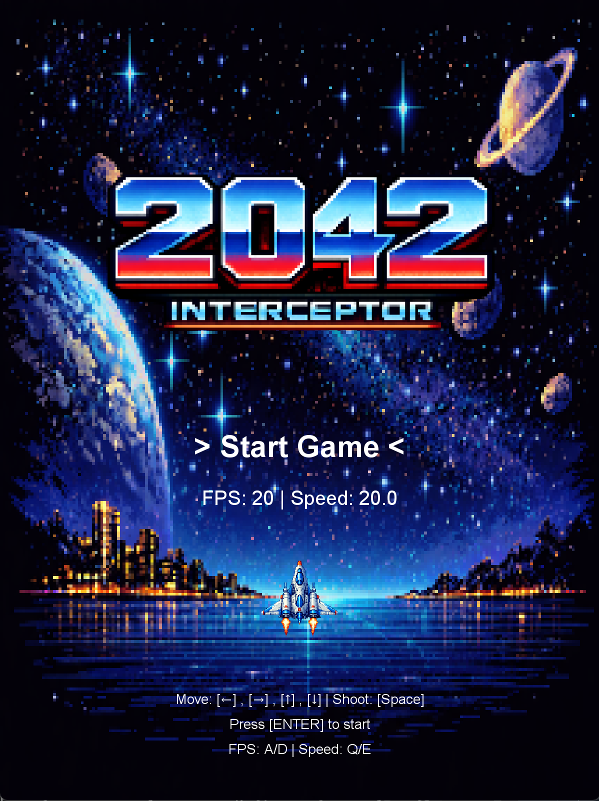
\includegraphics[width=0.5\linewidth]{../assets/title_screenshot.png} 
  \caption{ 2042: Interceptor.}
  \label{fig:menu}
\end{figure}

The game was built using \textbf{Java} and the \textbf{StdDraw} library for all the graphics and animations. I focused on making the gameplay feel smooth by including a calibration system for the frame rate and movement speed. This ensures that the experience stays consistent and challenging, regardless of the hardware it is running on.

\section{Game Dynamics}

\subsection{Stage 1: Main Menu}

\begin{figure}[H] % [H] forces the image to stay exactly here
  \centering
  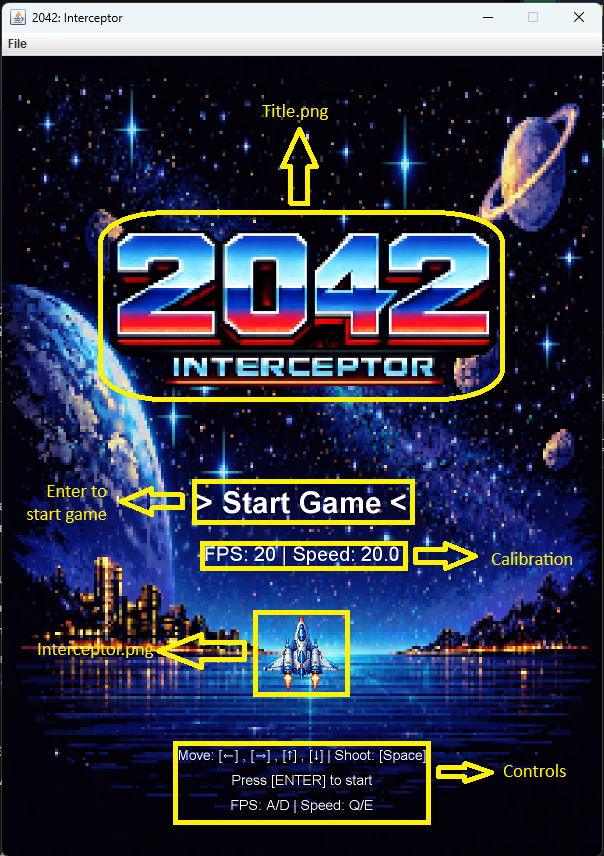
\includegraphics[width=0.7\linewidth]{../assets/menu_screenshot.png} 
  \caption{Main menu showing FPS and speed calibration options.} 
  \label{fig:menu}
\end{figure}

The main menu serves as an interactive calibration screen (as shown in Figure 2). It allows the player to test the game's mechanics and adjust performance settings before the mission begins.



\begin{itemize}
    \item \textbf{Visuals:} The menu renders three main assets: background.png, title.png, and interceptor.png.
    \item \textbf{Start Game:} Players use \key{ENTER} to start the game. 
    \item \textbf{Calibration:} \key{A}/\key{D} can be used to adjust FPS and \key{Q}/\key{E} to modify ship speed.
    \item \textbf{Testing:} The interceptor is fully controllable in the menu, using arrow keys to move and \key{SPACEBAR} to shoot, to allow for real-time testing of the settings.
    
\end{itemize}

\subsection{Stage 2: Gameplay}
The core gameplay involves navigating the interceptor to avoid enemy fire while the primary goal is to destroy the enemy fleet. When the interceptor or its bullet collides with an enemy, the enemy is destroyed, the score increases by 30 points, and an explosion animation is played. Conversely, when an enemy bullet or ship collides with the interceptor, one life is lost; when all lives are lost, the game is over.

\begin{figure}[H]
  \centering
  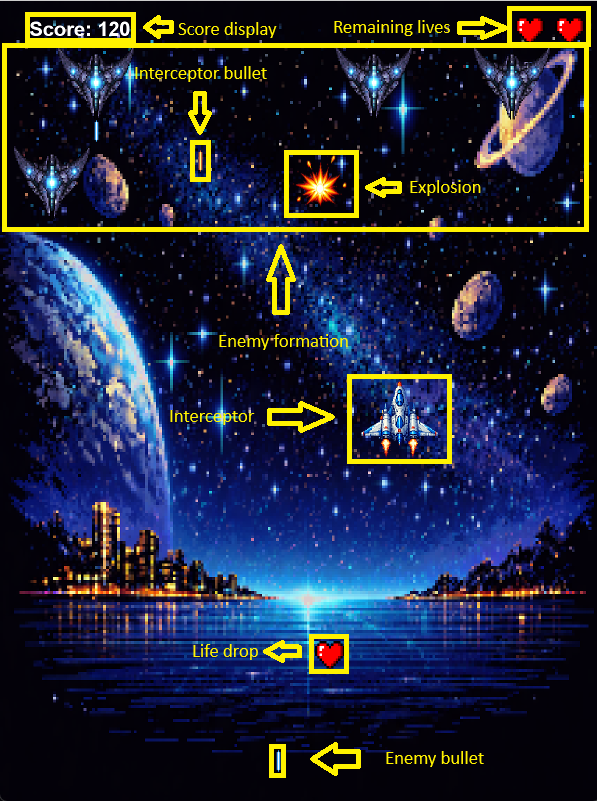
\includegraphics[width=0.7\linewidth]{../assets/gameplay_screenshot.png} 
  \caption{Active gameplay.} 
  \label{fig:gameplay}
\end{figure}

\subsubsection{Enemy Shooting Mechanics}
Each enemy has an internal cooldown and a random chance for shooting bullets, both of which can be adjusted according to the required difficulty. 

\begin{itemize}
    \item \textbf{Cooldown:} The cooldown is defined in seconds (\texttt{ENEMY\_SHOOT\_COOLDOWN}) and then multiplied by the current FPS. This ensures that the physical time a player must wait between enemy shots remains constant, regardless of the frame rate settings(as shown in Listing 1).
    \item \textbf{Random Chance:}To keep the difficulty uniform, the shooting probability is normalized by dividing the target chance per second by the current FPS. A shot is only triggered if a random value generated using \texttt{Math.random()} is lower than this adjusted threshold.
\end{itemize}

\begin{lstlisting}[caption={Randomized Enemy Shooting Logic}, label={lst:enemy_shoot}]
// Enemy Shooting: Divide chance by FPS to keep probability consistent per second
double adjustedShootChance = TARGET_SHOOT_CHANCE_PER_SEC / FPS;

if (Math.random() < adjustedShootChance && enemyShootCounter[i] == 0) {
    for (int j = 0; j < maxBullets; j++) {
        if (!bulletActive[j]) {
            bulletActive[j] = true;
            bulletX[j] = enemyX[i];
            bulletY[j] = enemyY[i] - HALF_ENEMY_HEIGHT;
            bulletDirection[j] = false; // Enemy bullets move DOWN
            enemyShootCounter[i] = (int) (ENEMY_SHOOT_COOLDOWN * FPS);
            break;
        }
    }
}
\end{lstlisting}

\subsubsection{Enemies Movement Mechanics}
The alien ships are arranged in layers and move horizontally. When any ship in a row hits the canvas boundary, the entire row reverses direction. To ensure the game feels consistent regardless of the hardware, movement speeds are normalized based on the current FPS(as shown in Listing 2).

\begin{lstlisting}[caption={Normalized Enemy Movement Logic}, label={lst:enemy_move}]
// BASE_SPEED is adjusted by FPS to ensure consistent distance over time
double normalizedEnemySpeed = (BASE_ENEMY_SPEED * 20.0) / FPS;
if (enemyDirection[i]) {
    enemyX[i] += normalizedEnemySpeed;
} else {
    enemyX[i] -= normalizedEnemySpeed;
}
\end{lstlisting}

\subsubsection{Collision Detection}
Every entity in the game has a rectangular hitbox, so collision detection is performed using simple mathematics. By adding the half-width and half-height of an entity to its center position, we can define a bounding rectangle; when two of these rectangles overlap, a collision is detected(as shown in Listing 3).

\begin{figure}[H]
  \centering
  % Resize the figure by adjusting the 0.6 value (60% of text width)
  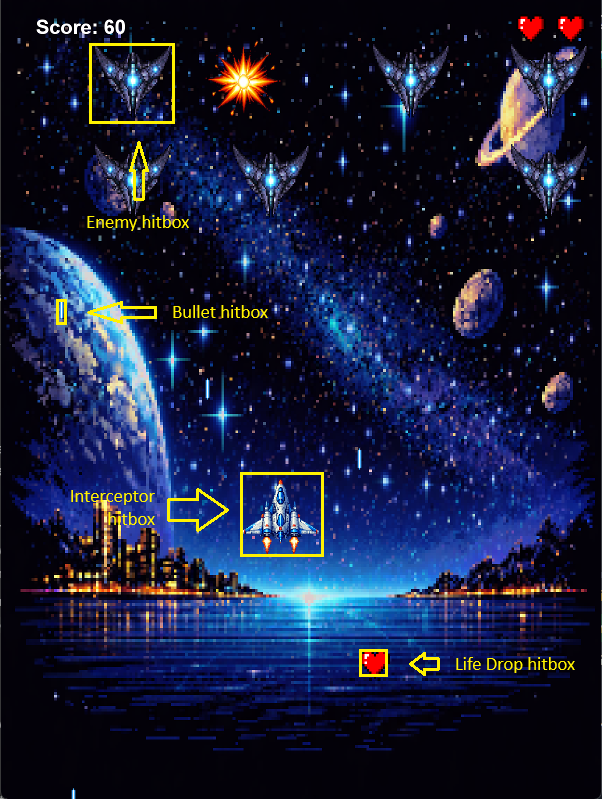
\includegraphics[width=0.6\textwidth]{../assets/collision_screenshot.png} 
  \caption{Bounding-box visualization for game entities.}
  \label{fig:bounding_box}
\end{figure}

\begin{lstlisting}[caption={AABB Collision Logic}, label={lst:collision}]
// Logic for checking overlap between two rectangles 
if (bulletX[i] + HALF_BULLET_WIDTH > enemyX[j] - HALF_ENEMY_WIDTH &&
    bulletX[i] - HALF_BULLET_WIDTH < enemyX[j] + HALF_ENEMY_WIDTH &&
    bulletY[i] + HALF_BULLET_HEIGHT > enemyY[j] - HALF_ENEMY_HEIGHT &&
    bulletY[i] - HALF_BULLET_HEIGHT < enemyY[j] + HALF_ENEMY_HEIGHT) {
    // Collision detected
    }
\end{lstlisting}

\subsubsection{Life Drop Mechanism}
To reward players and sustain gameplay, a probabilistic "Life Drop" mechanic is implemented. When an alien ship is destroyed, there is a randomized chance that a heart icon will spawn at the enemy's last coordinates. The decision to drop a life is determined by comparing a value from \texttt{Math.random()} against the \texttt{LIFE\_DROP\_CHANCE} constant(as shown in Listing 4).


\begin{lstlisting}[caption={Life Drop Logic on Enemy Destruction}, label={lst:life_drop}]
// Drop life heart if probability check passes (20% chance)
if (Math.random() < LIFE_DROP_CHANCE) {
    for (int k = 0; k < lifeDropActive.length; k++) {
        if (!lifeDropActive[k]) {
            lifeDropX[k] = enemyX[j];
            lifeDropY[k] = enemyY[j] - HALF_ENEMY_HEIGHT;
            lifeDropActive[k] = true;
            break;
        }
    }
}
\end{lstlisting}

\subsubsection{Pause Game}
When the player presses \key{P}, the game is instantly paused, freezing all entity movements and logic updates. While paused, a overlay is displayed, and the player has the option of resuming the game by pressing \key{P} again or returning to the main menu by pressing \key{ENTER}.

\begin{figure}[H]
  \centering
  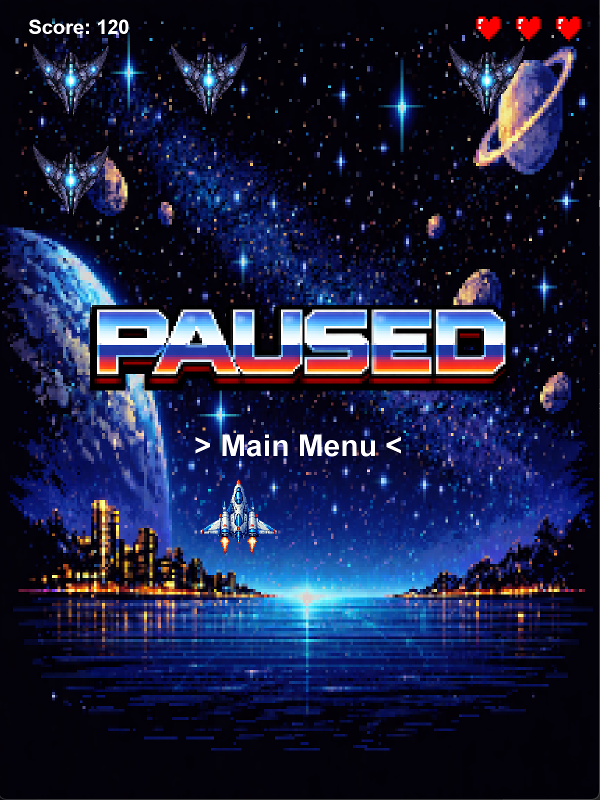
\includegraphics[width=0.65\textwidth]{../assets/paused_screenshot.png} 
  \caption{The pause screen overlay during gameplay.}
  \label{fig:pause}
\end{figure}

\subsection{Stage 3: End-Game}
The game concludes when the player either destroys all enemies or loses all three lives. In both scenarios, the final score is displayed along with navigation options to either restart the session or exit the application.

\subsubsection{Victory Case}
The victory screen is triggered once the player destroys all 8 alien ships, reaching a total score of 240. The screen displays the \texttt{victory.png} asset and provides the final score of the mission.

\begin{figure}[H]
  \centering
  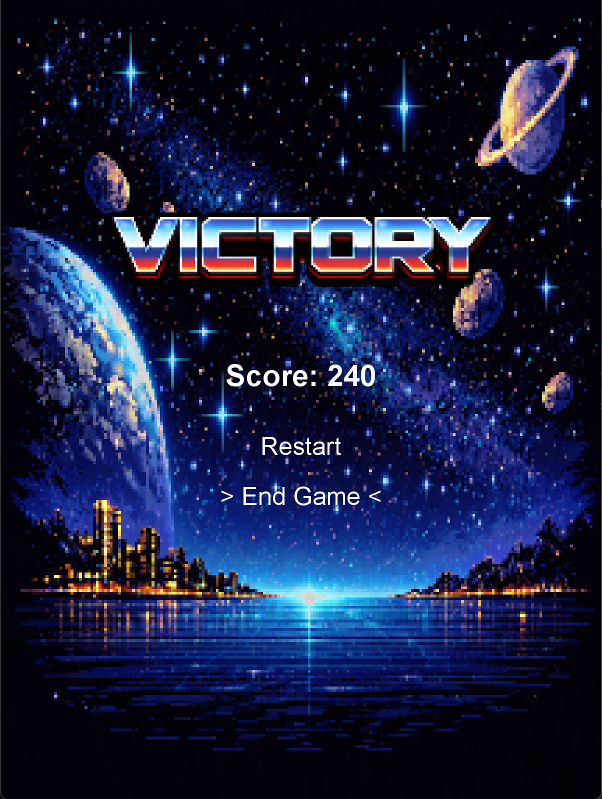
\includegraphics[width=0.7\linewidth]{../assets/victory_screenshot.png} 
  \caption{Victory screen with final score and navigation options.}
  \label{fig:victory}
\end{figure}

\subsubsection{Game Over Case}
If the player's life count reaches zero due to collisions with bullets or enemy ships, the "Game Over" screen is initiated. This screen utilizes the \texttt{gameOver.png} asset and shows the score achieved before defeat.

\begin{figure}[H]
  \centering
  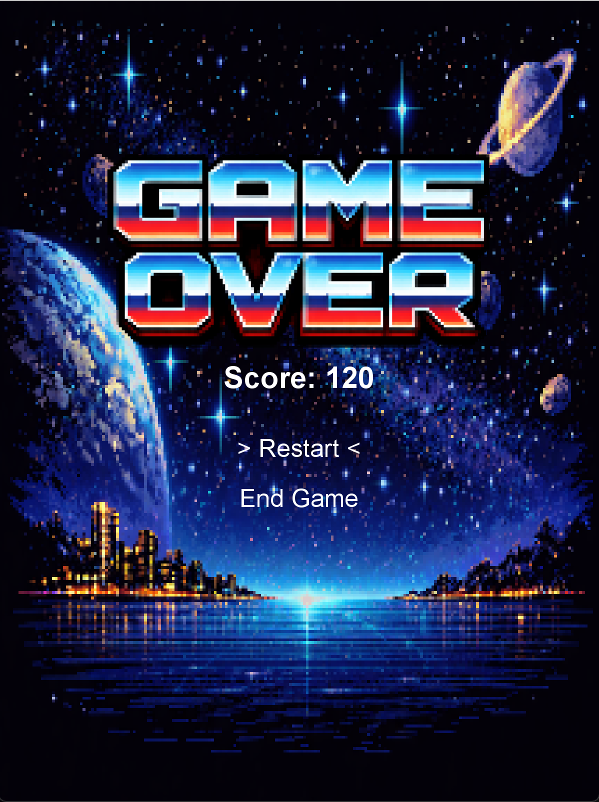
\includegraphics[width=0.7\linewidth]{../assets/gameover_screenshot.png} 
  \caption{Game Over screen displayed when the player loses all lives.}
  \label{fig:gameover}
\end{figure}

\subsubsection{Navigation and Selection}
On both end-game screens, the player can navigate between \textbf{Restart} and \textbf{End Game} options:
\begin{itemize}
    \item \textbf{Controls:} Navigation is handled using the $\uparrow$ and $\downarrow$ arrow keys.
    \item \textbf{Visual Feedback:} The current selection is emphasized with bold text and the \texttt{> <} symbols.
    \item \textbf{Execution:} Pressing \key{ENTER} confirms the selection. Choosing "Restart" resets the game state while keeping the previously calibrated FPS and speed settings, while "End Game" closes the window.
\end{itemize}

\section{Conclusion}
The development of \textit{2042: Interceptor} provided significant insights into the fundamental principles of game loop management, real-time input handling, and collision physics. By utilizing the \textbf{StdDraw} library within a procedural Java framework, I was able to implement a responsive and visually consistent arcade experience.
\end{document}